\documentclass{article}
\usepackage[T1]{fontenc}
\usepackage{hyperref}
\usepackage{amsmath}
\usepackage[utf8]{inputenc}
\usepackage[polish]{babel}
\usepackage{graphicx}
\usepackage{amsfonts}
\usepackage{placeins}


\setlength{\textheight}{21cm}

\title{{\bf Zadanie nr 1 - Generacja sygnału i szumu}\linebreak
Cyfrowe Przetwarzanie Sygnałów}
\author{Dominik Gałkowski, 247659 \and Jan Śladowski, 247806}
\date{25.03.2025}

\begin{document}
\clearpage\maketitle
\thispagestyle{empty}
\newpage
\setcounter{page}{1}
\section{Cel zadania}

Celem zadania jest stworzenie aplikacji do generowania sygnałów i szumów o określonych
przez użytkownika parametrach. Aplikacja ma posiadać możliowść wyświetlenia wykresów oraz histogramów,
zapisu i odczytu sygnałów, wykonania operacji na sygnałach oraz obliczenia parametrów sygnału.

\section{Wstp teoretyczny}

Program został stworzony w języku Python. Graficzny interfejs użytkownika został stworzony
przy wykorzystaniu bibliteki Tkinter. Do generowania wykresów i histogramów wykorzystana jest biblioteka Matplotlib,
natomiast do obliczeń wykorzystywana jest bibliotek Numpy. Program został podzielony na kilka plików.
Interfejs graficzny znajduje sie w głównym pliku - front. W plikach continousSignal oraz discretSignal znajdują
metody służące do obliczania sygnałów. Obliczanie parametrów sygnału znajduje sie w pliku calculateParams, a
metody odpowiedzialne za obsługe operacji na sygnałach umieszczone są w pliku signalOperation.

\subsection{Pełny interfejs uytkownika} 




Powyższy zrzut ekranu przedstawia panel interfejsu użytkownika. Po lewej stronie
            została umieszczona część odpowiedzialna za obsługę wykresów oraz dobór parametrów
            generowanego wykresu. Po prawej stronie została umieszczona część odpowiedzialna za
            wyświetlanie wygenerowanych wekresów, histogramów oraz parametrów. Interfejs zapewnia
            możliwość dodawanie dwóch wykresów.
\FloatBarrier
\begin{figure}[h!]
    \centering
    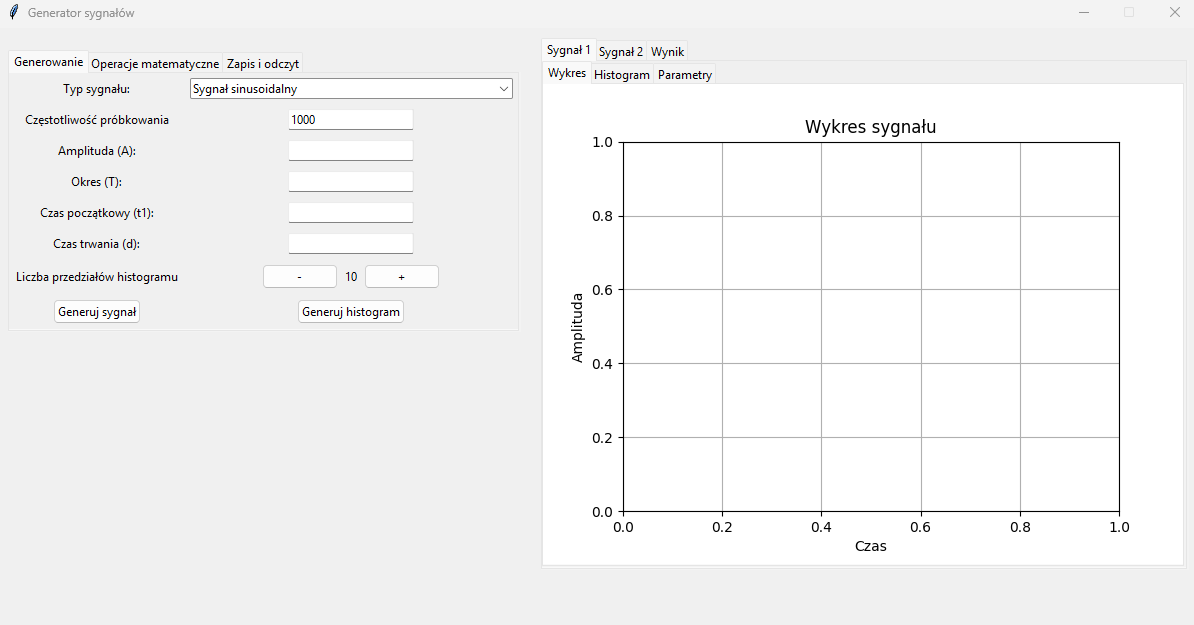
\includegraphics[width=\textwidth]{img/glowny.png}
    \caption{Pełny interfejs użytkownika}
\end{figure}

\subsection{Panel obsługi programu}  


Panel obsługi posiada 3 karty, które poprzez nacisniecie myszy można przełączać.
Pierwsza z nich oznaczona jako Generowanie odpowiada za wybór parametrów generowanego
wykresu, druga oznaczona jako Operacje matemtayczne pozwala na wybór operacji np. dodawanie, odejmowanie, mnożenie,
dzielenie, natomiast trzecia oznaczona jako Zapis i odczyt odpowiada za zapis, odczyt z pliku,
oraz wyświetlenie danych znajdujących sie w pliku.
\FloatBarrier
\begin{figure}[h!]
    \centering
    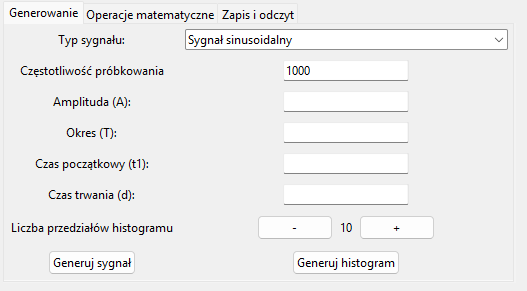
\includegraphics[width=\textwidth]{img/generuj.png}
    \caption{Panel wyboru parametrów}
\end{figure}
\FloatBarrier
\begin{figure}[h!]
    \centering
    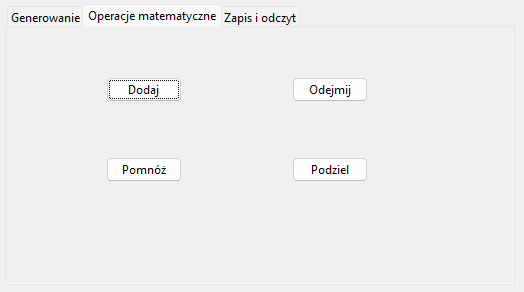
\includegraphics[width=\textwidth]{img/operacje.png}
    \caption{Panel wyboru operacji}
\end{figure}
\FloatBarrier
\begin{figure}[h!]
    \centering
    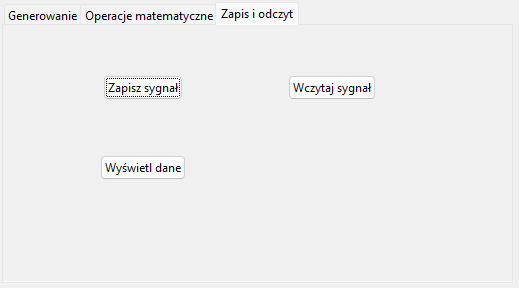
\includegraphics[width=\textwidth]{img/zapis.png}
    \caption{Panel zapisu i odczytu}
\end{figure}

\FloatBarrier
\subsection{Panel wyników} 

Panel wyników składa się z trzech kart: Sygnał 1, Sygnał 2 oraz Wynik. W pierszych dwóch kartach można
edytować wykresy, natomiast w trzeciej karcie pojawia się wynik operacji na sygnałach
Każda karta zwiera 3 sekcje: Wykres, Histogram oraz Parametry. W sekcji Wykres zostaje wyswietlony wygenerowany
wykres,w sekcji Histogram zostaje wyświetlony wygenerowany histogram natomiast w sekcji Parametry 
zostają wyświetlone parametry wykresu.

\begin{figure}[h!]
    \centering
    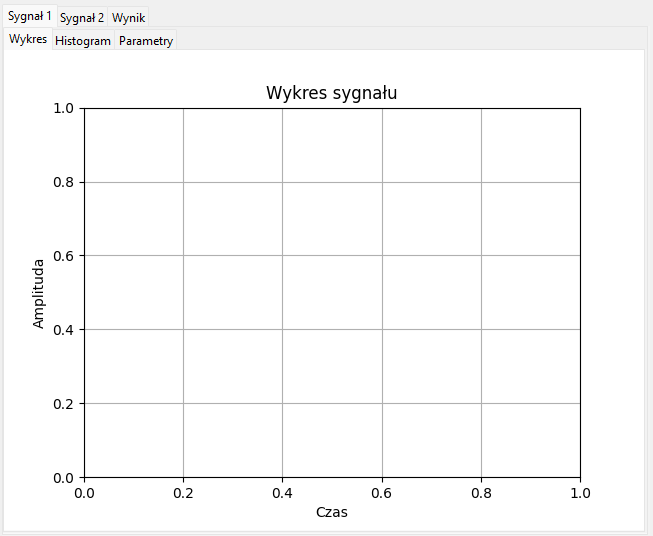
\includegraphics[width=\textwidth]{img/wykres.png}
    \caption{Karta wykresu}
\end{figure}
\begin{figure}[h!]
    \centering
    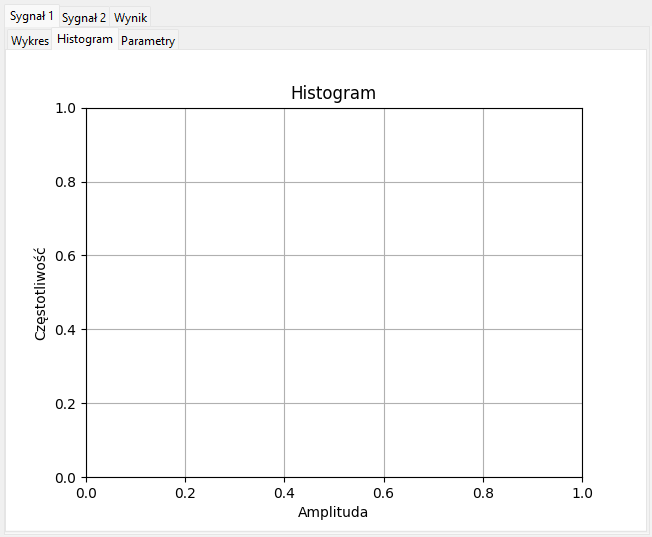
\includegraphics[width=\textwidth]{img/hist.png}
    \caption{Karta histogramu}
\end{figure}
\begin{figure}[h!]
    \centering
    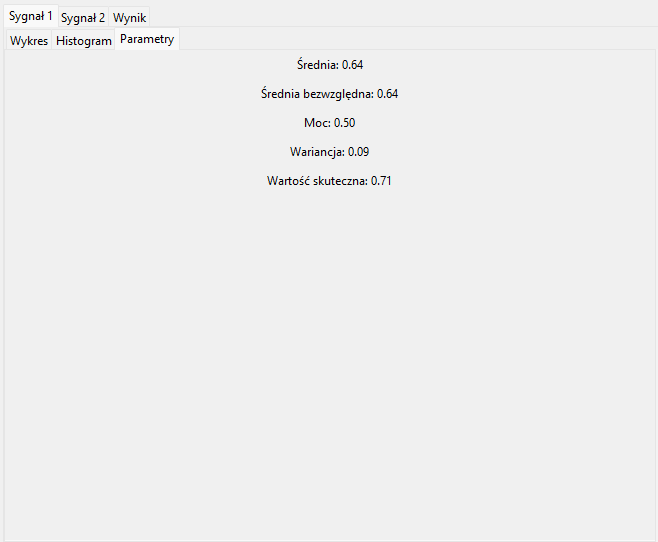
\includegraphics[width=\textwidth]{img/param.png}
    \caption{Karta wyliczonych parametrów}
\end{figure}
\FloatBarrier
\subsection{Wybór sygnałów do operacji} 


Po wybraniu operacji pojawia się dodatkowe okno, w którym można 
wybrać sygnały jakie maja być użyte do wykonania operacji.
\FloatBarrier
\begin{figure}[h!]
    \centering
    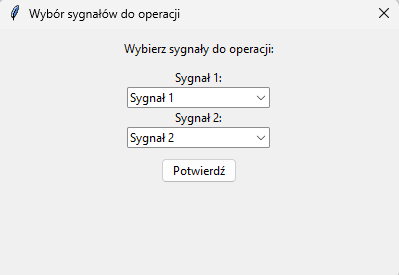
\includegraphics[width=\textwidth]{img/wybor.png}
    \caption{Wybór sygnałów do operacji}
\end{figure}




\section{Eksperymenty i wyniki}

Opis wykonywanych eksperymentw. Wymagane jest ilustrowanie przeprowadzanych dowiadcze wykresami oraz tabelami.

%%%%%%%%%%%%%%%%%%%%%%%%%%%%%%%%%%%%%%%%%%%%%%%%%%%%%%%%%%%%%%%%%%%%%%%%%%%%%%%%%%%%%%%%%%%%%%%%%%%%%%%%%%%%%%%%%
% PODROZDZIA� PT. EKSPERYMENT NR 1 
%%%%%%%%%%%%%%%%%%%%%%%%%%%%%%%%%%%%%%%%%%%%%%%%%%%%%%%%%%%%%%%%%%%%%%%%%%%%%%%%%%%%%%%%%%%%%%%%%%%%%%%%%%%%%%%%%

\subsection{Szum o rozkładzie jednostajnym} \label{szumjednostajny} 
    Celem eksperymentu było wygenerowanie szumu o rozkładzie jednostajnym o wybranych parametrach,
    które zostały opisane w sekcji założenia.

    
        Wykresy zostały wygenerowane przez losowe wartości z zakresu \[<-A_{max}, A_{max}>\]
        z jednakowym prawdopodobieństwem
    \noindent
    \subsubsection{Założenia}
    Parametry:
    
    \begin{table}[h!]
        \centering
        \vspace{0.2cm}
        \begin{tabular}{|c|c|}
            \hline\hline\\[-0.4cm]
            Amplitiuda & 1  \\
            \hline
            Czas początkowy & 0s  \\
            \hline
            Czas trwania sygnału & 5s  \\
            \hline
            Próbkowanie & 250Hz \\
            \hline
        \end{tabular}
        \caption{Parametry}
        \label{szumjednostajny}
    \end{table}
    \FloatBarrier
\subsubsection{Rezultat}
    \begin{figure}[h!]
        \centering
        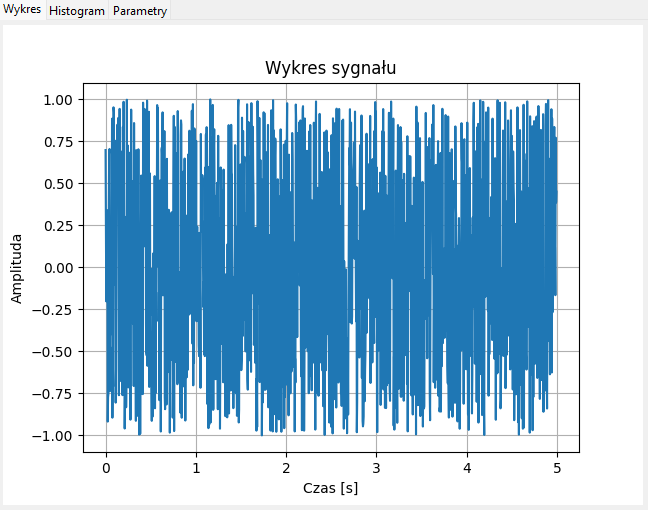
\includegraphics[width=\textwidth]{img/szum-jednost/wykres.png}
        \caption{Wykres}
    \end{figure}

    \begin{figure}[h!]
        \centering
        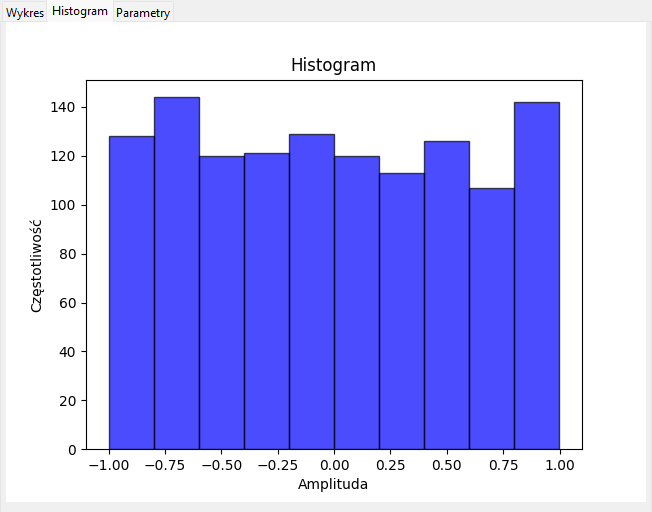
\includegraphics[width=\textwidth]{img/szum-jednost/hist.png}
        \caption{Histogram}
    \end{figure}
    \FloatBarrier
    Wyliczone parametry:
    \begin{table}[h!]
        \centering
        \vspace{0.2cm}
        \begin{tabular}{|c|c|}
            \hline\hline\\[-0.4cm]
            Średnia & 0.023  \\
            \hline
            Średnia bezwzględna & 0.510  \\
            \hline
            Moc średnia & 0.324  \\
            \hline
            Wariancja & 0.324 \\
            \hline
            Wartość skuteczna & 0.585 \\
            \hline
        \end{tabular}
        \caption{Wyliczone parametry}
        \label{szumjednostajny}
    \end{table}

\subsection{Szum gaussowski} \label{szumgaussowski} 
        Celem eksperymentu było wygenerowanie szumu gaussowskiego o wybranych parametrach,
        ktore zostały opisane w sekcji założenia. Funkcja opisująca sygnał:

        \begin{figure}[!htbp]
            \centering
            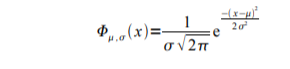
\includegraphics[width=0.5\textwidth]{img/szumgauss.png}
        \end{figure}
        \subsubsection{Założenia}
        \noindent
        Parametry:
        \begin{table}[h!]
            \centering
            \vspace{0.2cm}
            \begin{tabular}{|c|c|}
                \hline\hline\\[-0.4cm]
                Amplitiuda & 1  \\
                \hline
                Czas początkowy & 0s  \\
                \hline
                Czas trwania sygnału & 5s  \\
                \hline
                Próbkowanie & 250Hz \\
                \hline
            \end{tabular}
            \caption{Parametry}
            \label{szumgaussowski}
        \end{table}
    \subsubsection{Rezultat}
        \begin{figure}[h!]
            \centering
            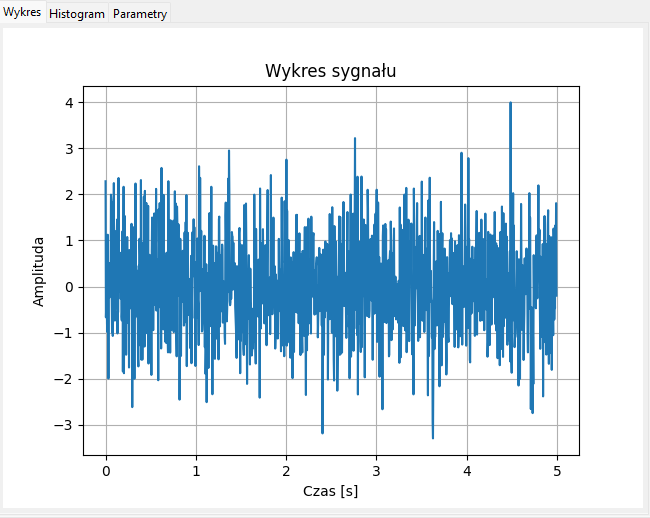
\includegraphics[width=\textwidth]{img/szum-gauss/wykres.png}
            \caption{Wykres}
        \end{figure}

        \begin{figure}[h!]
            \centering
            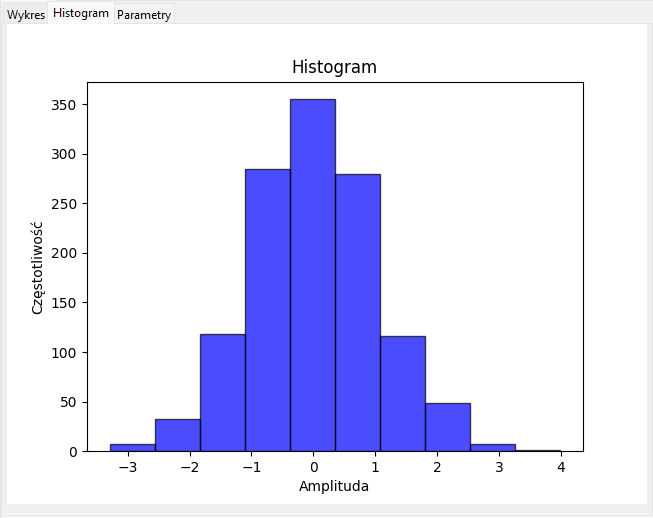
\includegraphics[width=\textwidth]{img/szum-gauss/hist.png}
            \caption{Histogram}
        \end{figure}
        \FloatBarrier
        Wyliczone parametry:
        \begin{table}[h!]
            \centering
            \vspace{0.2cm}
            \begin{tabular}{|c|c|}
                \hline\hline\\[-0.4cm]
                Średnia & 0.006  \\
                \hline
                Średnia bezwzględna & 0.791  \\
                \hline
                Moc średnia & 0.992  \\
                \hline
                Wariancja & 0.992 \\
                \hline
                Wartość skuteczna & 0.996 \\
                \hline
            \end{tabular}
            \caption{Wyliczone parametry}
            \label{szumgaussowski}
        \end{table}

\subsection{Sygnał sinusoidalny} \label{sinus} 
Celem eksperymentu było wygenerowanie sygnału sinusoidalnego o wybranych parametrach,
które zostały opisane w sekcji założenia. Funkcja opisująca sygnał:

\begin{figure}[!htbp]
    \centering
    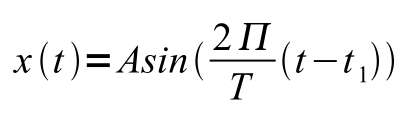
\includegraphics[width=0.6\textwidth]{img/sinus.png}
\end{figure}
\subsubsection{Założenia}
\noindent
Parametry:
\begin{table}[h!]
    \centering
    \vspace{0.2cm}
    \begin{tabular}{|c|c|}
        \hline\hline\\[-0.4cm]
        Amplitiuda & 1  \\
        \hline
        Czas początkowy & 0s  \\
        \hline
        Czas trwania sygnału & 4s  \\
        \hline
        Próbkowanie & 1000Hz \\
        \hline
        Okres & 1s\\
        \hline
    \end{tabular}
    \caption{Parametry}
    \label{sinus}
\end{table}
\subsubsection{Rezultat}
\begin{figure}[h!]
    \centering
    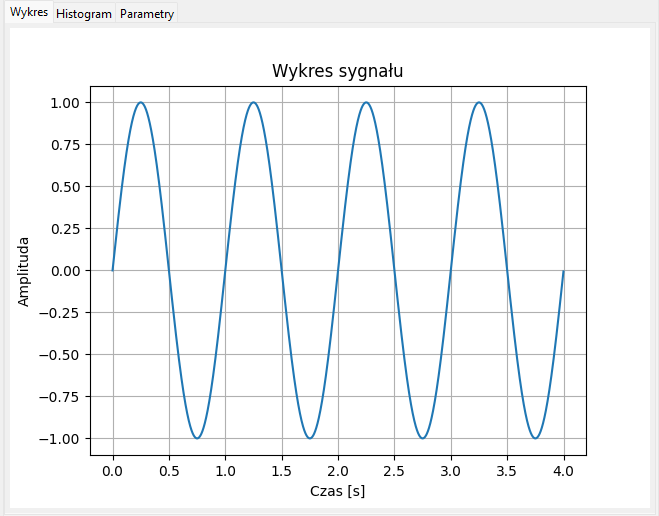
\includegraphics[width=\textwidth]{img/sinus/wykres.png}
    \caption{Wykres}
\end{figure}

\begin{figure}[h!]
    \centering
    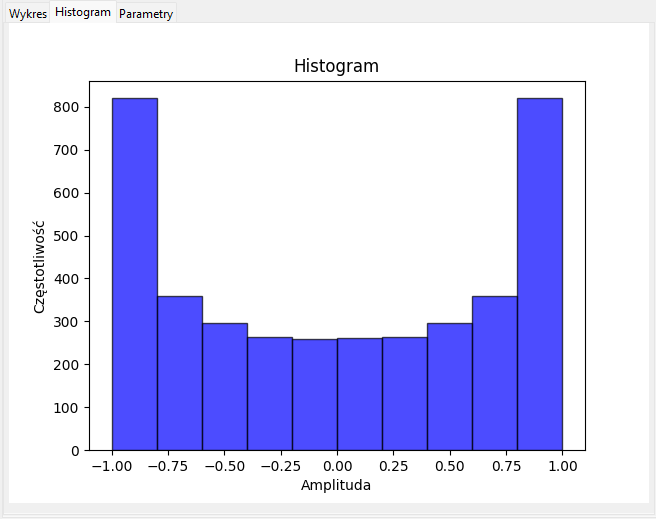
\includegraphics[width=\textwidth]{img/sinus/hist.png}
    \caption{Histogram}
\end{figure}
\FloatBarrier
Wyliczone parametry:
\begin{table}[h!]
    \centering
    \vspace{0.2cm}
    \begin{tabular}{|c|c|}
        \hline\hline\\[-0.4cm]
        Średnia & 0.000  \\
        \hline
        Średnia bezwzględna & 0.637  \\
        \hline
        Moc średnia & 0.500  \\
        \hline
        Wariancja & 0.500 \\
        \hline
        Wartość skuteczna & 0.707 \\
        \hline
    \end{tabular}
    \caption{Wyliczone parametry}
    \label{sinus}
\end{table}

\subsection{Sygnał sinusoidalny wyprostowany jednopołówkowo} \label{sinusjednopolowkowy} 
Celem eksperymentu było wygenerowanie sygnału sinusoidalnego wyprostowanego jednopołówkowo o wybranych parametrach,
które zostały opisane w sekcji założenia. Funkcja opisująca sygnał:

\begin{figure}[!htbp]
    \centering
    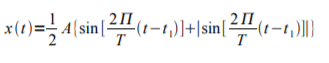
\includegraphics[width=0.6\textwidth]{img/sinusjedno.png}
\end{figure}
\subsubsection{Założenia}
\noindent
Parametry:
\begin{table}[h!]
    \centering
    \vspace{0.2cm}
    \begin{tabular}{|c|c|}
        \hline\hline\\[-0.4cm]
        Amplitiuda & 1  \\
        \hline
        Czas początkowy & 0s  \\
        \hline
        Czas trwania sygnału & 4s  \\
        \hline
        Próbkowanie & 1000Hz \\
        \hline
        Okres & 1s\\
        \hline
    \end{tabular}
    \caption{Parametry}
    \label{sinusjednopolowkowy}
\end{table}
\subsubsection{Rezultat}
\begin{figure}[h!]
    \centering
    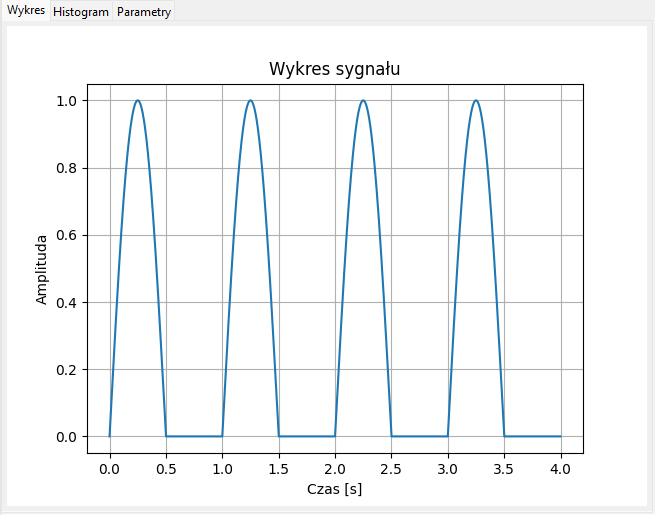
\includegraphics[width=\textwidth]{img/sinus-jedno/wykres.png}
    \caption{Wykres}
\end{figure}

\begin{figure}[h!]
    \centering
    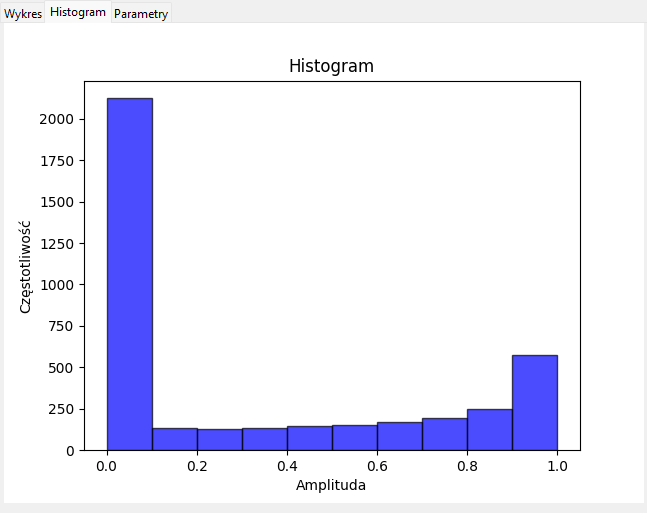
\includegraphics[width=\textwidth]{img/sinus-jedno/hist.png}
    \caption{Histogram}
\end{figure}
\FloatBarrier
Wyliczone parametry:
\begin{table}[h!]
    \centering
    \vspace{0.2cm}
    \begin{tabular}{|c|c|}
        \hline\hline\\[-0.4cm]
        Średnia & 0.318  \\
        \hline
        Średnia bezwzględna & 0.318  \\
        \hline
        Moc średnia & 0.250  \\
        \hline
        Wariancja & 0.149 \\
        \hline
        Wartość skuteczna & 0.500 \\
        \hline
    \end{tabular}
    \caption{Wyliczone parametry}
    \label{sinusjednopolowkowy}
\end{table}

\subsection{Sygnał sinusoidalny wyprostowany dwupołówkowo} \label{sinusdwupolowkowy} 
Celem eksperymentu było wygenerowanie sygnału sinusoidalnego wyprostowanego dwupołówkowo o wybranych parametrach,
które zostały opisane w sekcji założenia. Funkcja opisująca sygnał:

\begin{figure}[!htbp]
    \centering
    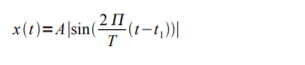
\includegraphics[width=0.6\textwidth]{img/sinusdwu.png}
\end{figure}
\subsubsection{Założenia}
\noindent
Parametry:
\begin{table}[h!]
    \centering
    \vspace{0.2cm}
    \begin{tabular}{|c|c|}
        \hline\hline\\[-0.4cm]
        Amplitiuda & 1  \\
        \hline
        Czas początkowy & 0s  \\
        \hline
        Czas trwania sygnału & 4s  \\
        \hline
        Próbkowanie & 1000Hz \\
        \hline
        Okres & 1s\\
        \hline
    \end{tabular}
    \caption{Parametry}
    \label{sinusdwupolowkowy}
\end{table}
\subsubsection{Rezultat}
\begin{figure}[h!]
    \centering
    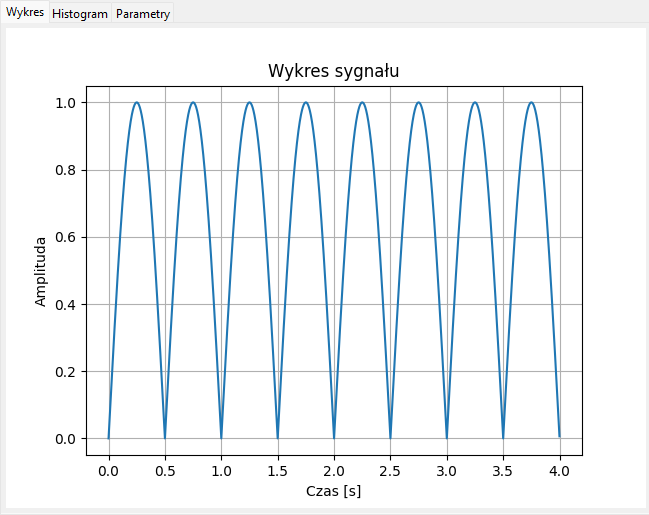
\includegraphics[width=\textwidth]{img/sinus-dwu/wykres.png}
    \caption{Wykres}
\end{figure}

\begin{figure}[h!]
    \centering
    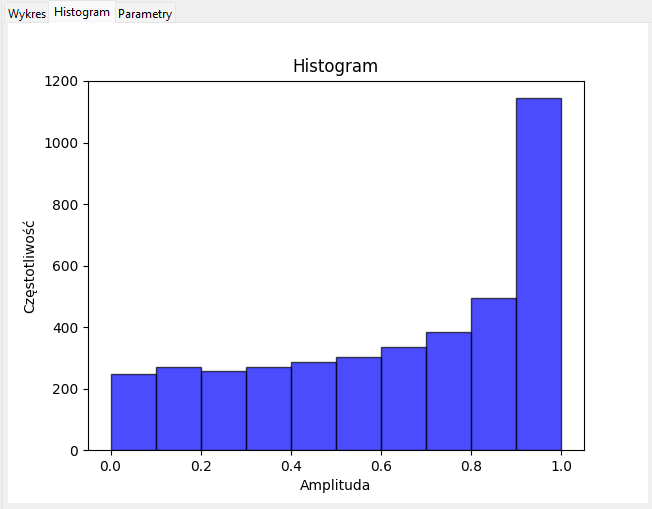
\includegraphics[width=\textwidth]{img/sinus-dwu/hist.png}
    \caption{Histogram}
\end{figure}
\FloatBarrier
Wyliczone parametry:
\begin{table}[h!]
    \centering
    \vspace{0.2cm}
    \begin{tabular}{|c|c|}
        \hline\hline\\[-0.4cm]
        Średnia & 0.637  \\
        \hline
        Średnia bezwzględna & 0.637  \\
        \hline
        Moc średnia & 0.500  \\
        \hline
        Wariancja & 0.095 \\
        \hline
        Wartość skuteczna & 0.707 \\
        \hline
    \end{tabular}
    \caption{Wyliczone parametry}
    \label{sinusdwupolowkowy}
\end{table}

\subsection{Sygnał prostokątny} \label{prostokat} 
Celem eksperymentu było wygenerowanie prostokątnego o wybranych parametrach,
które zostały opisane w sekcji założenia. Funkcja opisująca sygnał:

\begin{figure}[!htbp]
    \centering
    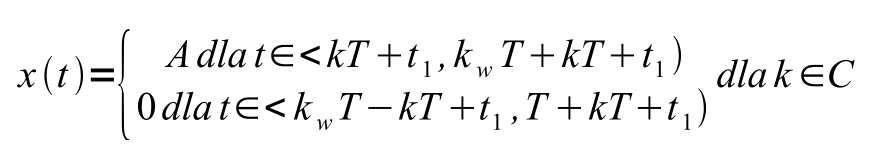
\includegraphics[width=0.7\textwidth]{img/prostokat.png}
\end{figure}
\subsubsection{Założenia}
\noindent
Parametry:
\begin{table}[h!]
    \centering
    \vspace{0.2cm}
    \begin{tabular}{|c|c|}
        \hline\hline\\[-0.4cm]
        Amplitiuda & 1  \\
        \hline
        Czas początkowy & 0s  \\
        \hline
        Czas trwania sygnału & 4s  \\
        \hline
        Próbkowanie & 1000Hz \\
        \hline
        Okres & 1s\\
        \hline
        Współczynnik wypełnienia & 0.75\\
        \hline
    \end{tabular}
    \caption{Parametry}
    \label{prostokat}
\end{table}
\subsubsection{Rezultat}
\begin{figure}[h!]
    \centering
    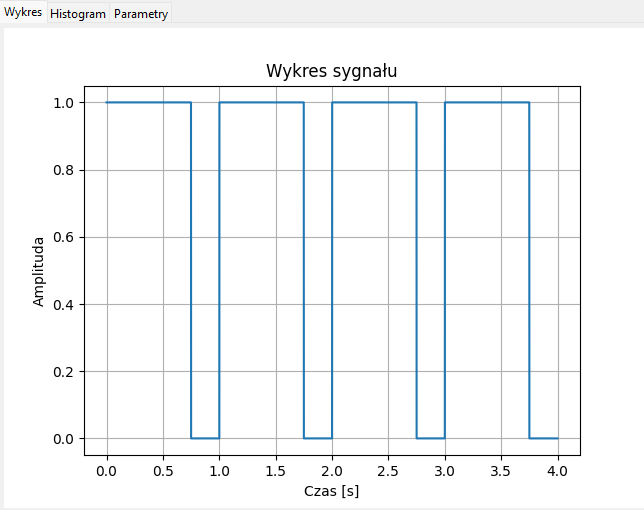
\includegraphics[width=\textwidth]{img/prostokat/wykres.png}
    \caption{Wykres}
\end{figure}

\begin{figure}[h!]
    \centering
    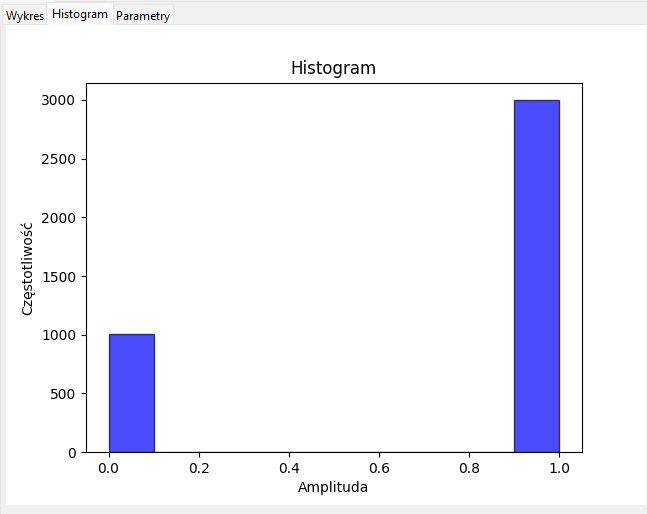
\includegraphics[width=\textwidth]{img/prostokat/hist.png}
    \caption{Histogram}
\end{figure}
\FloatBarrier
Wyliczone parametry:
\begin{table}[h!]
    \centering
    \vspace{0.2cm}
    \begin{tabular}{|c|c|}
        \hline\hline\\[-0.4cm]
        Średnia & 0.750  \\
        \hline
        Średnia bezwzględna & 0.750  \\
        \hline
        Moc średnia & 0.750  \\
        \hline
        Wariancja & 0.188 \\
        \hline
        Wartość skuteczna & 0.866 \\
        \hline
    \end{tabular}
    \caption{Wyliczone parametry}
    \label{prostokat}
\end{table}

\subsection{Sygnał prostokątny symetryczny} \label{prostokatsymetryczny} 
Celem eksperymentu było wygenerowanie sygnału prostokątnego symetryczne o wybranych parametrach,
które zostały opisane w sekcji założenia. Funkcja opisująca sygnał:

\begin{figure}[!htbp]
    \centering
    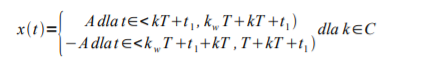
\includegraphics[width=0.7\textwidth]{img/prostokatsymet.png}
\end{figure}
\subsubsection{Założenia}
\noindent
Parametry:
\begin{table}[h!]
    \centering
    \vspace{0.2cm}
    \begin{tabular}{|c|c|}
        \hline\hline\\[-0.4cm]
        Amplitiuda & 1  \\
        \hline
        Czas początkowy & 0s  \\
        \hline
        Czas trwania sygnału & 4s  \\
        \hline
        Próbkowanie & 1000Hz \\
        \hline
        Okres & 1s\\
        \hline
        Współczynnik wypełnienia & 0.75\\
        \hline
    \end{tabular}
    \caption{Parametry}
    \label{prostokatsymetryczny}
\end{table}
\subsubsection{Rezultat}
\begin{figure}[h!]
    \centering
    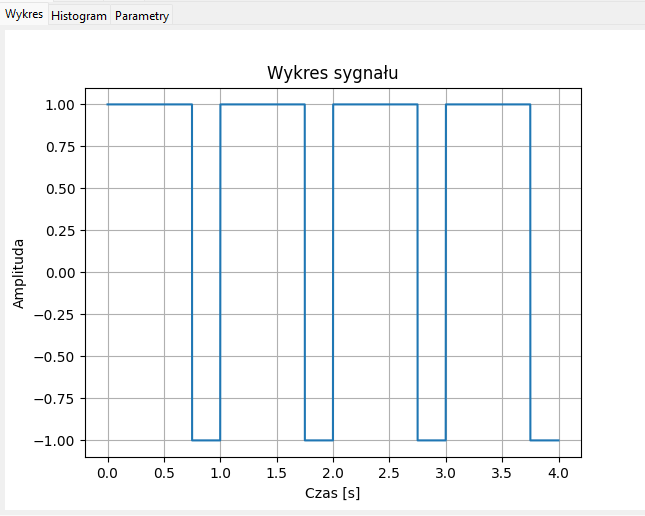
\includegraphics[width=\textwidth]{img/prostokatsymetryczny/wykres.png}
    \caption{Wykres}
\end{figure}

\begin{figure}[h!]
    \centering
    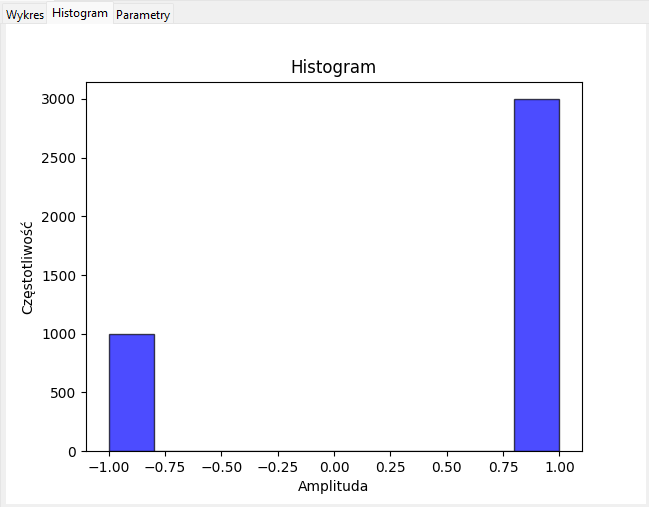
\includegraphics[width=\textwidth]{img/prostokatsymetryczny/hist.png}
    \caption{Histogram}
\end{figure}
\FloatBarrier
Wyliczone parametry:
\begin{table}[h!]
    \centering
    \vspace{0.2cm}
    \begin{tabular}{|c|c|}
        \hline\hline\\[-0.4cm]
        Średnia & 0.500  \\
        \hline
        Średnia bezwzględna & 0.999  \\
        \hline
        Moc średnia & 0.999  \\
        \hline
        Wariancja & 0.750 \\
        \hline
        Wartość skuteczna & 1.000 \\
        \hline
    \end{tabular}
    \caption{Wyliczone parametry}
    \label{prostokatsymetryczny}
\end{table}

\subsection{Sygnał trójkątny} \label{trojkat} 
Celem eksperymentu było wygenerowanie sygnału trójkątnego o wybranych parametrach,
które zostały opisane w sekcji założenia. Funkcja opisująca sygnał:

\begin{figure}[!htbp]
    \centering
    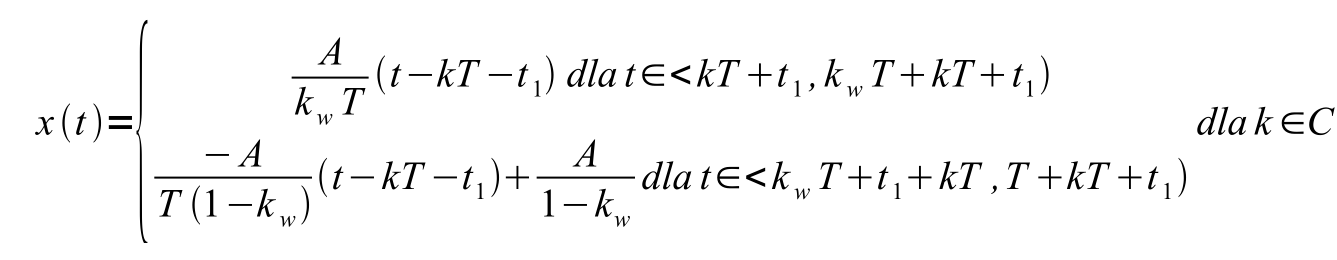
\includegraphics[width=0.7\textwidth]{img/trojkat.png}
\end{figure}
\subsubsection{Założenia}
\noindent
Parametry:
\begin{table}[h!]
    \centering
    \vspace{0.2cm}
    \begin{tabular}{|c|c|}
        \hline\hline\\[-0.4cm]
        Amplitiuda & 1  \\
        \hline
        Czas początkowy & 0s  \\
        \hline
        Czas trwania sygnału & 4s  \\
        \hline
        Próbkowanie & 1000Hz \\
        \hline
        Okres & 1s\\
        \hline
        Współczynnik wypełnienia & 0.75\\
        \hline
    \end{tabular}
    \caption{Parametry}
    \label{trojkat}
\end{table}
\subsubsection{Rezultat}
\begin{figure}[h!]
    \centering
    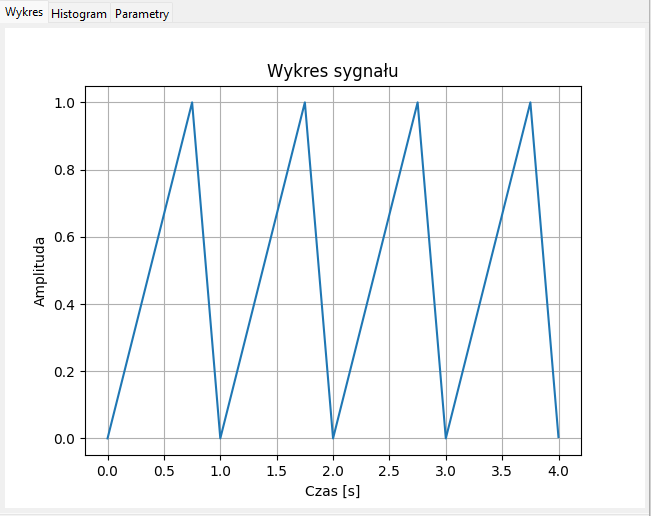
\includegraphics[width=\textwidth]{img/trojkat/wykres.png}
    \caption{Wykres}
\end{figure}

\begin{figure}[h!]
    \centering
    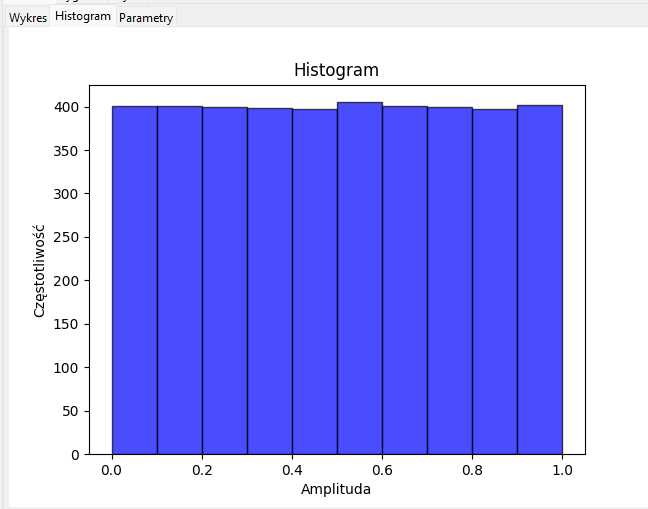
\includegraphics[width=\textwidth]{img/trojkat/hist.png}
    \caption{Histogram}
\end{figure}
\FloatBarrier
Wyliczone parametry:
\begin{table}[h!]
    \centering
    \vspace{0.2cm}
    \begin{tabular}{|c|c|}
        \hline\hline\\[-0.4cm]
        Średnia & 0.500  \\
        \hline
        Średnia bezwzględna & 0.500  \\
        \hline
        Moc średnia & 0.333  \\
        \hline
        Wariancja & 0.083 \\
        \hline
        Wartość skuteczna & 0.577 \\
        \hline
    \end{tabular}
    \caption{Wyliczone parametry}
    \label{trojkat}
\end{table}     

\subsection{Skok jednostkowy} \label{skokjednostowy} 
Celem eksperymentu było wygenerowanie skoku jednostkowego o wybranych parametrach,
                które zostały opisane w sekcji założenia. Funkcja opisująca sygnał:

        \begin{figure}[!htbp]
            \centering
            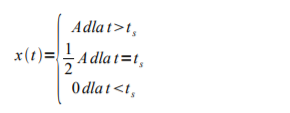
\includegraphics[width=0.5\textwidth]{img/skokjednostowy.png}
        \end{figure}
\subsubsection{Założenia}
\noindent
Parametry:
\begin{table}[h!]
    \centering
    \vspace{0.2cm}
    \begin{tabular}{|c|c|}
        \hline\hline\\[-0.4cm]
        Amplitiuda & 1  \\
        \hline
        Czas początkowy & 0s  \\
        \hline
        Czas trwania sygnału & 4s  \\
        \hline
        Próbkowanie & 1000Hz \\
        \hline
        Czsa skoku & 1s\\
        \hline
    \end{tabular}
    \caption{Parametry}
    \label{skokjednostowy}
\end{table}
\subsubsection{Rezultat}
\begin{figure}[h!]
    \centering
    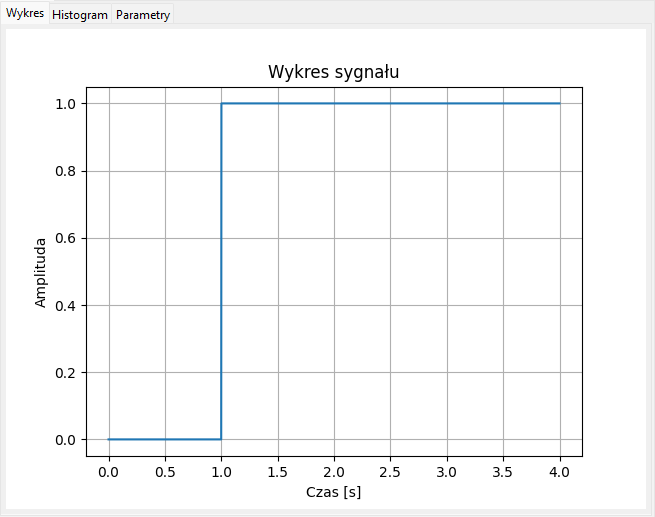
\includegraphics[width=\textwidth]{img/skok/wykres.png}
    \caption{Wykres}
\end{figure}

\begin{figure}[h!]
    \centering
    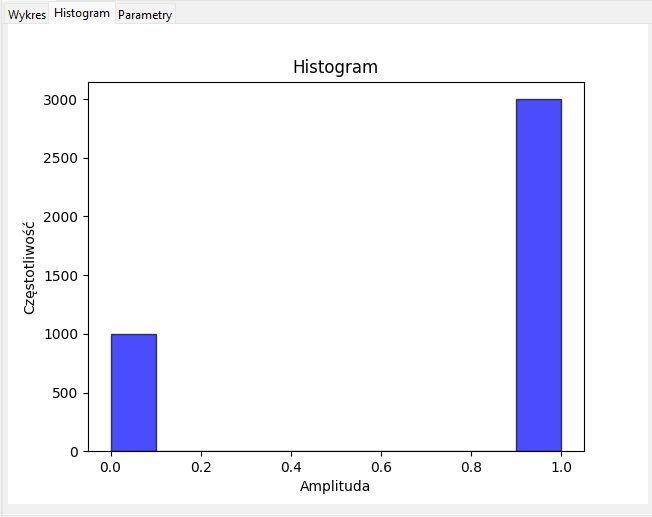
\includegraphics[width=\textwidth]{img/skok/hist.png}
    \caption{Histogram}
\end{figure}
\FloatBarrier
Wyliczone parametry:
\begin{table}[h!]
    \centering
    \vspace{0.2cm}
    \begin{tabular}{|c|c|}
        \hline\hline\\[-0.4cm]
        Średnia & 0.750  \\
        \hline
        Średnia bezwzględna & 0.750  \\
        \hline
        Moc średnia & 0.750  \\
        \hline
        Wariancja & 0.187 \\
        \hline
        Wartość skuteczna & 0.866 \\
        \hline
    \end{tabular}
    \caption{Wyliczone parametry}
    \label{skokjednostowy}
\end{table}     

\subsection{Impuls jednostkowy} \label{impuls} 
Celem eksperymentu było wygenerowanie impulsu jednostkowego o wybranych parametrach,
ktore zostały opisane w sekcji założenia. Funkcja opisująca sygnał:

\begin{figure}[!htbp]
    \centering
    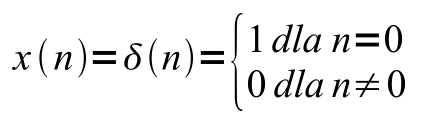
\includegraphics[width=0.3\textwidth]{img/impuls-jednostkowy.png}
\end{figure}
\subsubsection{Założenia}
\noindent
Parametry:
\begin{table}[h!]
    \centering
    \vspace{0.2cm}
    \begin{tabular}{|c|c|}
        \hline\hline\\[-0.4cm]
        Amplitiuda & 1  \\
        \hline
        Czas początkowy & 0s  \\
        \hline
        Czas trwania sygnału & 4s  \\
        \hline
        Próbkowanie & 10Hz \\
        \hline
        Czsa skoku & 1s\\
        \hline
    \end{tabular}
    \caption{Parametry}
    \label{impuls}
\end{table}
\subsubsection{Rezultat}
\begin{figure}[h!]
    \centering
    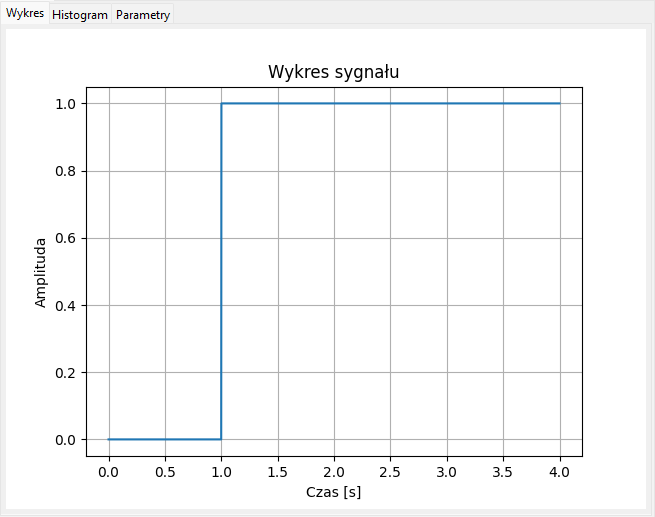
\includegraphics[width=\textwidth]{img/skok/wykres.png}
    \caption{Wykres}
\end{figure}

\begin{figure}[h!]
    \centering
    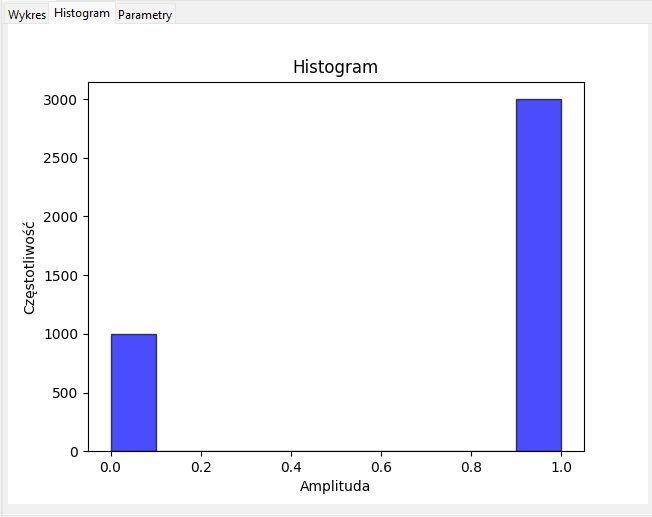
\includegraphics[width=\textwidth]{img/skok/hist.png}
    \caption{Histogram}
\end{figure}
\FloatBarrier
Wyliczone parametry:
\begin{table}[h!]
    \centering
    \vspace{0.2cm}
    \begin{tabular}{|c|c|}
        \hline\hline\\[-0.4cm]
        Średnia & 0.025  \\
        \hline
        Średnia bezwzględna & 0.025  \\
        \hline
        Moc średnia & 0.025  \\
        \hline
        Wariancja & 0.024 \\
        \hline
        Wartość skuteczna & 0.158 \\
        \hline
    \end{tabular}
    \caption{Wyliczone parametry}
    \label{impuls}
\end{table}  

\subsection{Szum impulsowy} \label{szumimpuls} 
Celem eksperymentu było wygenerowanie szumu impulsowego o wybranych parametrach,
ktore zostały opisane w sekcji założenia.
\subsubsection{Założenia}
\noindent
Parametry:
\begin{table}[h!]
    \centering
    \vspace{0.2cm}
    \begin{tabular}{|c|c|}
        \hline\hline\\[-0.4cm]
        Amplitiuda & 1  \\
        \hline
        Czas początkowy & 0s  \\
        \hline
        Czas trwania sygnału & 4s  \\
        \hline
        Próbkowanie & 10Hz \\
        \hline
        Prawdopodobieństwo & 0.5\\
        \hline
    \end{tabular}
    \caption{Parametry}
    \label{szumimpuls}
\end{table}
\FloatBarrier
\subsubsection{Rezultat}
\begin{figure}[h!]
    \centering
    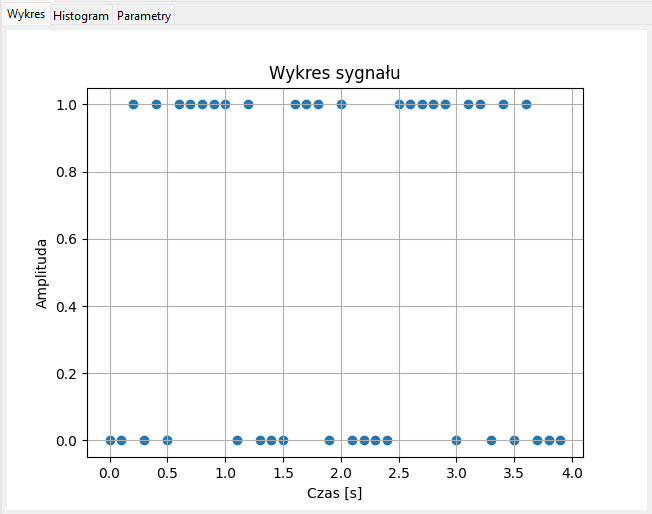
\includegraphics[width=\textwidth]{img/szum-impuls/wykres.png}
    \caption{Wykres}
\end{figure}

\begin{figure}[h!]
    \centering
    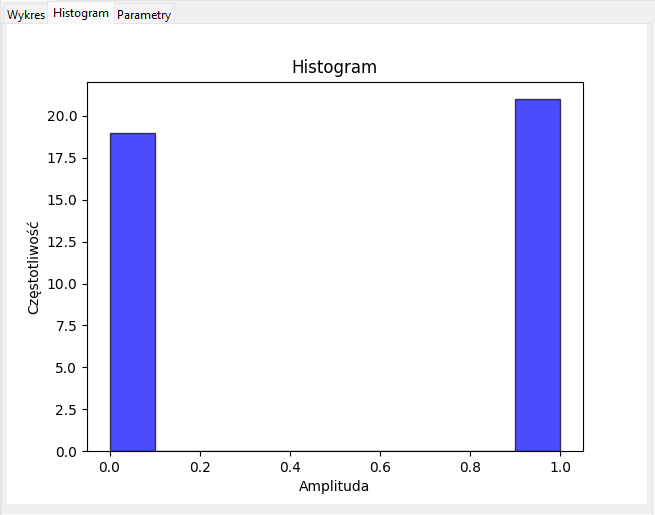
\includegraphics[width=\textwidth]{img/szum-impuls/hist.png}
    \caption{Histogram}
\end{figure}
\FloatBarrier
Wyliczone parametry:
\begin{table}[h!]
    \centering
    \vspace{0.2cm}
    \begin{tabular}{|c|c|}
        \hline\hline\\[-0.4cm]
        Średnia & 0.525  \\
        \hline
        Średnia bezwzględna & 0.525  \\
        \hline
        Moc średnia & 0.525  \\
        \hline
        Wariancja & 0.249 \\
        \hline
        Wartość skuteczna & 0.725 \\
        \hline
    \end{tabular}
    \caption{Wyliczone parametry}
    \label{szumimpuls}
\end{table}  

\subsection{Dodawanie sygnałów} \label{add} 
Celem eksperymentu było dodanie sygnałów, które zostały opisane w sekcji założenia

\subsubsection{Założenia} 
    Parametry wykresów zostały określone w eksperymencie |3.6| oraz |3.8|


\subsubsection{Rezultat}
\begin{figure}[h!]
    \centering
    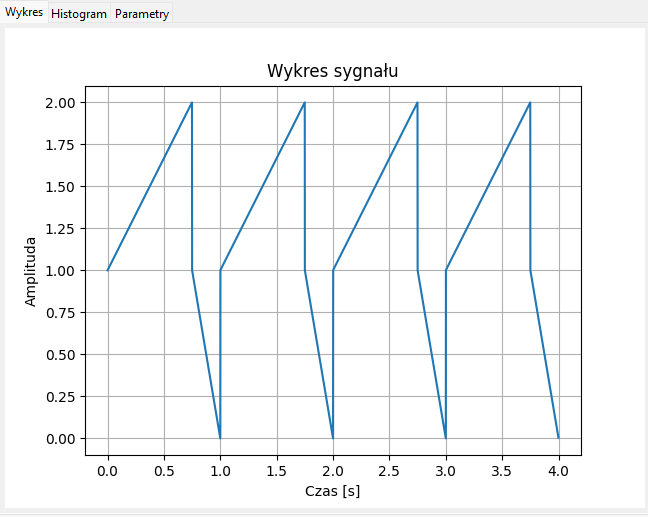
\includegraphics[width=\textwidth]{img/add/wykres.png}
    \caption{Wykres}
\end{figure}

\begin{figure}[h!]
    \centering
    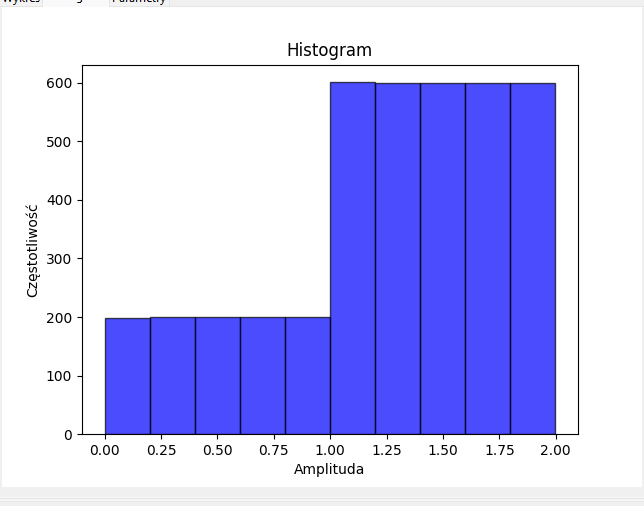
\includegraphics[width=\textwidth]{img/add/hist.png}
    \caption{Histogram}
\end{figure}
\FloatBarrier
Wyliczone parametry:
\begin{table}[h!]
    \centering
    \vspace{0.2cm}
    \begin{tabular}{|c|c|}
        \hline\hline\\[-0.4cm]
        Średnia & 1.250  \\
        \hline
        Średnia bezwzględna & 1.250  \\
        \hline
        Moc średnia & 1.833  \\
        \hline
        Wariancja & 0.271 \\
        \hline
        Wartość skuteczna & 1.354 \\
        \hline
    \end{tabular}
    \caption{Wyliczone parametry}
    \label{add}
\end{table}  

\subsection{Odejmowanie sygnałów} \label{sub} 
Celem eksperymentu było odejmowanie sygnałów, które zostały opisane w sekcji założenia

\subsubsection{Założenia} 
    Parametry wykresów zostały określone w eksperymencie |3.6| oraz |3.8|


\subsubsection{Rezultat}
\begin{figure}[h!]
    \centering
    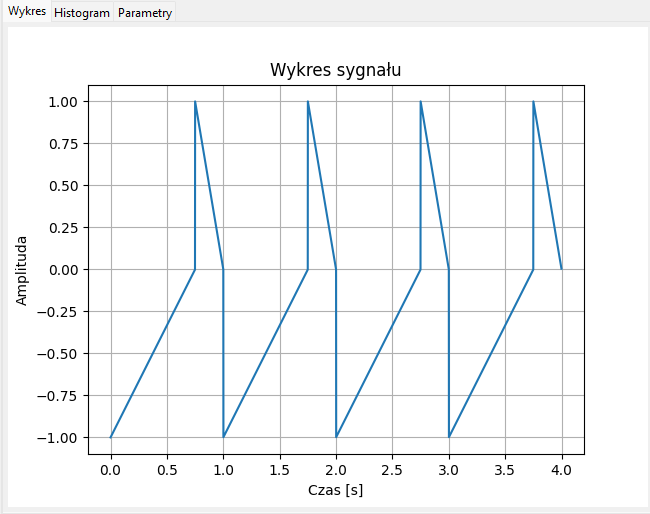
\includegraphics[width=\textwidth]{img/sub/wykres.png}
    \caption{Wykres}
\end{figure}

\begin{figure}[h!]
    \centering
    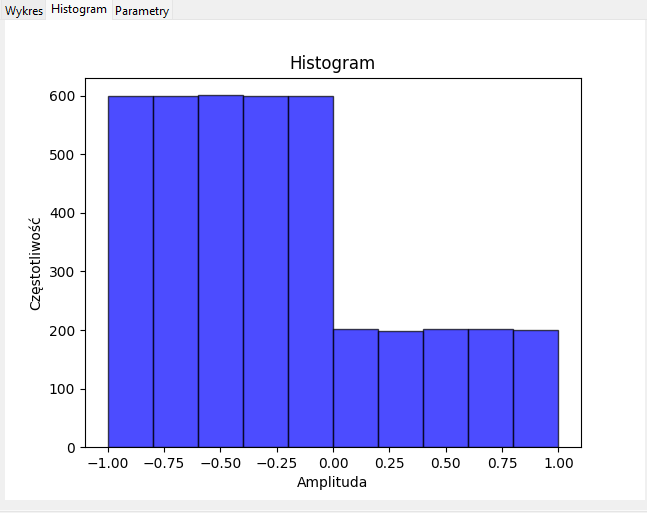
\includegraphics[width=\textwidth]{img/sub/hist.png}
    \caption{Histogram}
\end{figure}
\FloatBarrier
Wyliczone parametry:
\begin{table}[h!]
    \centering
    \vspace{0.2cm}
    \begin{tabular}{|c|c|}
        \hline\hline\\[-0.4cm]
        Średnia & -0.249  \\
        \hline
        Średnia bezwzględna & 0.500  \\
        \hline
        Moc średnia & 0.334  \\
        \hline
        Wariancja & 0.271 \\
        \hline
        Wartość skuteczna & 0.577 \\
        \hline
    \end{tabular}
    \caption{Wyliczone parametry}
    \label{sub}
\end{table} 

\subsection{Mnożenie sygnałów} \label{mul} 
Celem eksperymentu było mnożenie sygnałów, które zostały opisane w sekcji założenia

\subsubsection{Założenia} 
    Parametry wykresów zostały określone w eksperymencie |3.6| oraz |3.8|


\subsubsection{Rezultat}
\begin{figure}[h!]
    \centering
    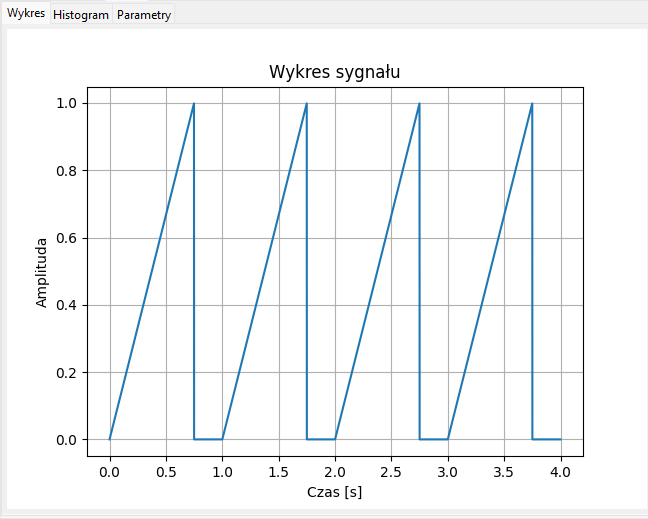
\includegraphics[width=\textwidth]{img/mul/wykres.png}
    \caption{Wykres}
\end{figure}

\begin{figure}[h!]
    \centering
    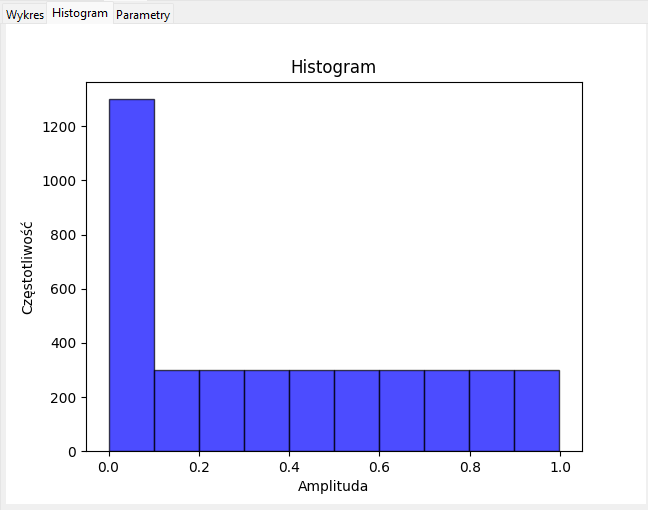
\includegraphics[width=\textwidth]{img/mul/hist.png}
    \caption{Histogram}
\end{figure}
\FloatBarrier
Wyliczone parametry:
\begin{table}[h!]
    \centering
    \vspace{0.2cm}
    \begin{tabular}{|c|c|}
        \hline\hline\\[-0.4cm]
        Średnia & 0.375 \\
        \hline
        Średnia bezwzględna & 0.375  \\
        \hline
        Moc średnia & 0.250  \\
        \hline
        Wariancja & 0.109 \\
        \hline
        Wartość skuteczna & 0.500 \\
        \hline
    \end{tabular}
    \caption{Wyliczone parametry}
    \label{mul}
\end{table}   

\subsection{Dzielenie sygnałów} \label{div} 

Celem eksperymentu było mnożenie sygnałów, które zostały opisane w sekcji założenia

\subsubsection{Założenia} 
    Parametry wykresów zostały określone w eksperymencie |3.6| oraz |3.8|


\subsubsection{Rezultat}
\begin{figure}[h!]
    \centering
    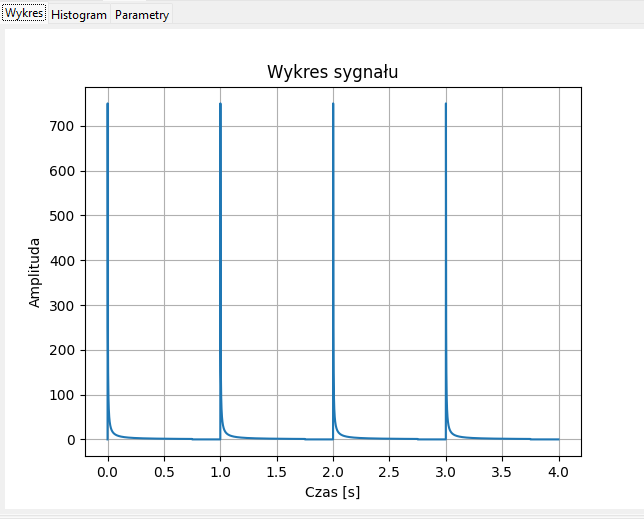
\includegraphics[width=\textwidth]{img/div/wykres.png}
    \caption{Wykres}
\end{figure}

\begin{figure}[h!]
    \centering
    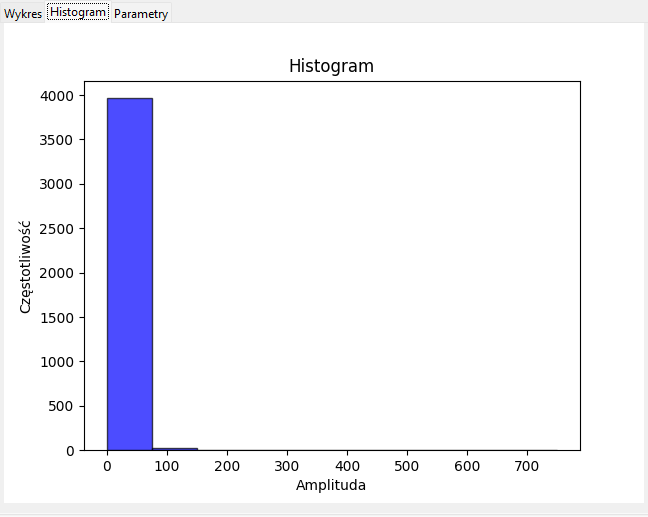
\includegraphics[width=\textwidth]{img/div/hist.png}
    \caption{Histogram}
\end{figure}
\FloatBarrier
Wyliczone parametry:
\begin{table}[h!]
    \centering
    \vspace{0.2cm}
    \begin{tabular}{|c|c|}
        \hline\hline\\[-0.4cm]
        Średnia & 5.572 \\
        \hline
        Średnia bezwzględna & 5.572  \\
        \hline
        Moc średnia & 1079.007  \\
        \hline
        Wariancja & 1047.987 \\
        \hline
        Wartość skuteczna & 32.848 \\
        \hline
    \end{tabular}
    \caption{Wyliczone parametry}
    \label{div}
\end{table}   

\section{Wnioski}
    Program został zaprojektowany i zaimplementowany zgodnie ze specyfikacją
    określoną w instrukcji, co gwarantuje jego zgodność z założeniami projektowymi. 
    Opracowane rozwiązanie umożliwia poprawne generowanie sygnałów, wykonywanie operacji 
    matematycznych oraz zapis i odczyt wygenerowanych wykresów.

    W procesie projektowania oraz implementacji szczególną uwagę poświęcono zapewnieniu 
    elastyczności i rozszerzalności kodu, co umożliwia jego łatwą adaptację do przyszłych 
    rozszerzeń oraz dodanie nowych funkcjonalności w kolejnych etapach realizacji projektu.
    

%%%%%%%%%%%%%%%%%%%%%%%%%%%%%%%%%%%%%%%%%%%%%%%%%%%%%%%%%%%%%%%%%%%%%%%%%%%%%%%%%%%%%%%%%%%%%%%%%%%%%%%%%%%%%%%%%
% BIBLIOGRAFIA
%%%%%%%%%%%%%%%%%%%%%%%%%%%%%%%%%%%%%%%%%%%%%%%%%%%%%%%%%%%%%%%%%%%%%%%%%%%%%%%%%%%%%%%%%%%%%%%%%%%%%%%%%%%%%%%%%

\begin{thebibliography}{9}

    \bibitem{instrukcja}
    Politechnika Łódzka, 
    \emph{Instrukcja do zadania 1}, 
    Dostęp online: \url{https://ftims.edu.p.lodz.pl/mod/url/view.php?id=6495}, 
    [dostęp: 24 marca 2025].


    \bibitem{python-doc}
    Python Software Foundation, 
    \emph{Python Documentation}, 
    Dostęp online: \url{https://docs.python.org/3/}, 
    [dostęp: 24 marca 2025].

    \bibitem{tkinter-doc}
    Python Software Foundation, 
    \emph{Tkinter Documentation}, 
    Dostęp online: \url{https://docs.python.org/3/library/tkinter.html}, 
    [dostęp: 24 marca 2025].

\end{thebibliography}

\end{document}
